\section{Introduction}

Deep feed-forward architectures have brought impressive advances to the state-of-the-art across a wide variety of machine-learning tasks and applications. At the moment, however, these leaps in performance come only when a large amount of labeled training data is available. At the same time, for problems lacking labeled data, it may be still possible to obtain training sets that are big enough for training large-scale deep models, but that suffer from the {\em shift} in data distribution from the actual data encountered at ``test time''. One particularly important example is synthetic or semi-synthetic training data, which may come in abundance and be fully labeled, but which inevitably have a distribution that is different from real data~\cite{Liebelt10,Stark10,Vazquez14,Sun14}.

%lucrative way for computer vision tasks, is to use computer graphics or some sort of image-based rendering to synthesize/augment labeled training sets.


%Deep feed-forward neural networks have shown remarkable results, advancing the state-of-the-art over a range of diverse application domains, starting from handwritten symbols recognition \cite{LeCun89}, including speech/signal recognition \cite{}, and most recently, computer vision \cite{Krizhevsky2012}. The appeal of deep feed-forward networks is the ability to obtain discrimination accuracy that is often unachievable with any other class of methods, while using fairly generic components and optimization algorithms during training. Due to this dependence on the large datasets, the progress with deep feed-forward networks as well as other large-scale discriminative learning architectures is largely dependent on finding new sources of training data. For example, in computer vision, a recurrent topic these days is the use of very large datasets of synthetic or ``semi''-synthetic imagery \cite{Kinect, INRIA}.

%Notably, in the case of each application domain, the key enabling factor for the success of deep discriminative learning was not the design of new architectures, but rather the availability of very large annotated datasets. In each case, the exact definition of ``very large'' depended on the complexity of the domain. 

 

%In many situations, it is possible to obtain large training sets that are big enough to be suitable for training large-scale deep models, but that also have significant {\em shifts} in data distributions between the available training data and the actual data encountered at ``test time''. E.g.\ in the example above, it might be possible to synthesize an almost infinite amount of synthetic images, however there will always be an inevitable disparity in the distribution of such synthetic images and real images that are of ultimate interest at test time. Consequently, a classifier or a structure predictor learned on synthetic data, while performing very well on the synthetic images, might perform sub-optimally on real images.

Learning a discriminative classifier or other predictor in the presence of a {\em shift} between training and test distributions is known as {\em domain adaptation} (DA). A number of approaches to domain adaptation has been suggested in the context of {\em shallow} learning, e.g.\ in the situation when data representation/features are given and fixed. The proposed approaches then build the mappings between the {\em source} (training-time) and the {\em target} (test-time) domains, so that the classifier learned for the source domain can also be applied to the target domain, when composed with the learned mapping between domains. The appeal of the domain adaptation approaches is the ability to learn a mapping between domains in the situation when the target domain data are either fully unlabeled ({\em unsupervised domain annotation}) or have few labeled samples ({\em semi-supervised domain adaptation}). Below, we focus on the harder unsupervised case, although the proposed approach can be generalized to the semi-supervised case rather straightforwardly.

Unlike most previous papers on domain adaptation that worked with fixed feature representations, we focus on combining domain adaptation and deep feature learning within one training process ({\em deep domain adaptation}). Our goal is to embed domain adaptation into the process of learning representation, so that the final classification decisions are made based on features that are both discriminative and invariant to the change of domains, i.e.\ have the same or very similar distributions in the source and the target domains. In this way, the obtained feed-forward network can be applicable to the target domain without being hindered by the shift between the two domains.

We thus focus on learning features that combine (i) discriminativeness and (ii) domain-invariance. This is achieved by jointly optimizing the underlying features as well as two discriminative classifiers operating on these features: (i) the \emph{label predictor} that predicts class labels and is used both during training and at test time and (ii) the \emph{domain classifier} that discriminates between the source and the target domains during training. While the parameters of the classifiers are optimized in order to minimize their error on the training set, the parameters of the underlying deep feature mapping are optimized in order to {\em minimize} the loss of the label classifier and to {\em maximize} the loss of the domain classifier. The latter encourages domain-invariant features to emerge in the course of the optimization.

\begin{figure*}

\centering
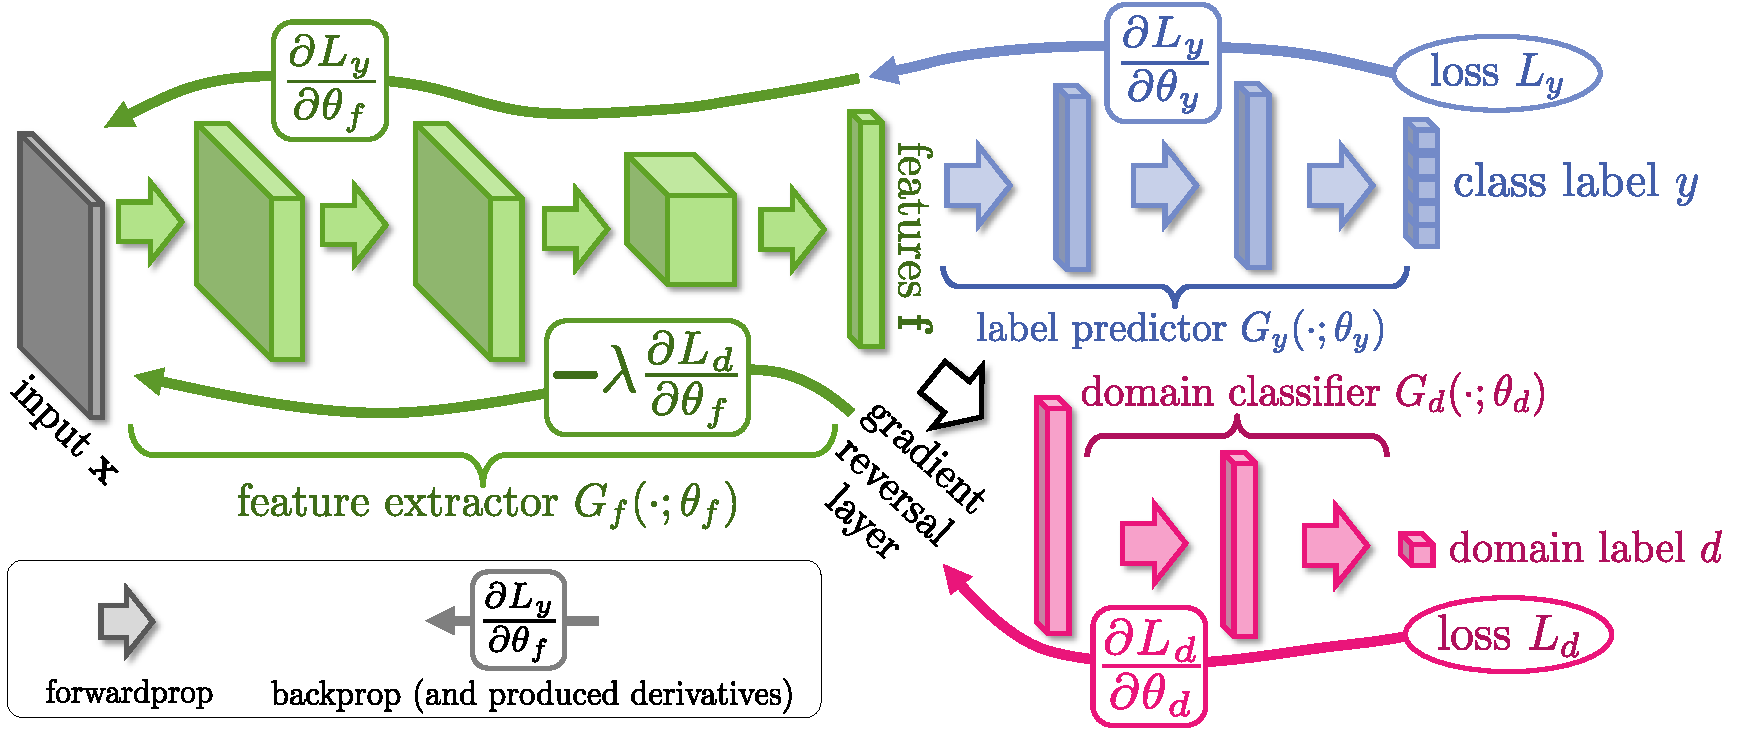
\includegraphics[width=0.8\textwidth]{figures/deepDA2.pdf}

\caption{The {\bf proposed architecture} includes a deep {\em feature extractor} (green) and a deep {\em label predictor} (blue), which together form a standard feed-forward architecture. Unsupervised domain adaptation is achieved by adding a {\em domain classifier} (red) connected to the feature extractor via a {\em gradient reversal layer} that multiplies the gradient by a certain negative constant during the backpropagation-based training. Otherwise, the training proceeds in a standard way and minimizes the label prediction loss (for source examples) and the domain classification loss (for all samples). Gradient reversal ensures that the feature distributions over the two domains are made similar (as indistinguishable as possible for the domain classifier), thus resulting in the domain-invariant features.\vspace{-2mm}}
\label{fig:arch}
\end{figure*}


Crucially, we show that all three training processes can be embedded into an appropriately composed deep feed-forward network (\fig{arch}) that uses standard layers and loss functions, and can be trained using standard backpropagation algorithms based on stochastic gradient descent or its modifications (e.g.\ SGD with momentum). Our approach is generic as it can be used to add domain adaptation to any existing feed-forward architecture that is trainable by backpropagation. In practice, the only non-standard component of the proposed architecture is a rather trivial {\em gradient reversal} layer that leaves the input unchanged during forward propagation and reverses the gradient by multiplying it by a negative scalar during the backpropagation.  

%As will be seen, such  layer allows the optimization process to mimimize the ability of the domain classifier to discriminate between the domains and ensures the domain-invariance of the deep features.

Below, we detail the proposed approach to domain adaptation in deep architectures, and present results on traditional deep learning image datasets (such as MNIST~\cite{LeCun98} and SVHN~\cite{Netzer11}) as well as on {\sc Office} benchmarks \cite{Saenko10}, where the proposed method considerably improves over previous state-of-the-art accuracy.




